\documentclass[a4paper]{article}

\usepackage[T2A]{fontenc}
\usepackage[utf8]{inputenc}
\usepackage[russian]{babel}
\usepackage{graphicx}
\usepackage{float}
\usepackage{mathtools}
\usepackage{wrapfig}
\usepackage{amsfonts, amssymb, amsmath, latexsym}
\usepackage{nicefrac}
\usepackage{hhline}
\usepackage{multirow}
\usepackage[colorlinks=true,linkcolor=blue,citecolor=blue]{hyperref}       % hyperlinks
\usepackage{nicefrac}       % compact symbols for 1/2, etc.
\usepackage{nameref}
\usepackage{booktabs}       % professional-quality tables
\usepackage{algorithm}
\usepackage{algpseudocode}
\usepackage{xcolor, colortbl}
\usepackage{etoolbox}

% \graphicspath{ {./} }

\usepackage[verbose=true,letterpaper]{geometry}

\newgeometry{
    textheight=25cm,
    textwidth=18cm,
    top=2.5cm,
    headheight=12pt,
    headsep=10pt,
    footskip=1cm,
    marginparwidth=15pt
}

%\usepackage{showframe} 

\usepackage{epigraph}
\usepackage{amsmath,amsfonts,amssymb,amsthm,mathtools, mathrsfs}
\usepackage{amsthm}

<<<<<<< HEAD
\title{Работа 4.4.3 \\ Изучение призмы с помощью гониометра}
=======
\title{Работа 4.5.2 \\ Интерференция лазерного излучения}
>>>>>>> 38d184f2ece362e4e0625fc2796df1bbefb7ea4b
\author{Шарапов Денис, Б05-005}
\date{}

\usepackage{fancyhdr}
\pagestyle{fancy}
\fancyhf{}
<<<<<<< HEAD
\rhead{Работа 4.4.3}
=======
\rhead{Работа 4.5.2}
>>>>>>> 38d184f2ece362e4e0625fc2796df1bbefb7ea4b
\lhead{}
\cfoot{\thepage}
\usepackage{subcaption}
\usepackage[font={small}]{caption}

\begin{document}

    \maketitle
    \tableofcontents
    \newpage
    
\section{Аннотация}

\noindent\textbf{Цель работы:} знакомство с работой и настройкой гониометра Г5, определение зависимости показателя преломления стекла призмы от длины волны, определение марки стекла и спектральных характеристик призмы. \smallskip
 
\noindent \textbf{В работе используются:} гониометр, ртутная лампа, призма.

\section{Теоретические сведения}

Показатель преломления материала призмы $n(\lambda)$ удобно определять
по углу наименьшего отклонения $\delta(\lambda)$ (рис. 1). Минимальное отклонение луча, преломлённого призмой, от направления луча, падающего
на призму, получается при симметричном ходе луча (в призме луч идёт
параллельно основанию). Угол минимального отклонения $\delta$, преломляющий угол $\alpha$ (угол при вершине призмы) и показатель преломления
связаны соотношением $$n(\lambda) = \frac{\sin{\frac{\alpha + \delta(\lambda)}{2}}}{\sin{\frac{\alpha}{2}}}.$$

\begin{figure}[ht!]
    \centering
    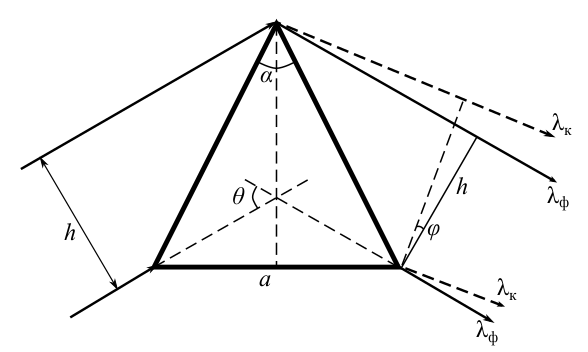
\includegraphics[width = 0.5\textwidth]{image/pic1.png}
    \caption{Ход лучей в призме для угла наименьшего отклонения}
\end{figure}

\section{Результаты измерений и обработка данных}

Измеренные углы наименьшего отклонения 6-ти ярких линий спектра ртути представлены в табл. 1. По этой таблице вычислим значение показателя преломления (табл. 2) и построим график (рис. 2). 

\begin{table}[!ht]
    \centering
    \caption{Результаты измерения наименьшего отклонения 6-ти ярких диний спектра ртути}
    \begin{tabular}{|c|c|c|c|c|c|c|c|}
    \hline
    K$_1$                 & K$_2$                 & $1$                   & $2$                   & $3$                   & $4$                   & $5$                   & $6$                   \\ \hline
    $86^{\circ} 02' 56''$ & $85^{\circ} 36' 31''$ & $85^{\circ} 34' 19''$ & $85^{\circ} 36' 01''$ & $85^{\circ} 29' 56''$ & $85^{\circ} 29' 14''$ & $85^{\circ} 13' 52''$ & $85^{\circ} 11' 21''$ \\ \hline
    \end{tabular}
    \end{table}

\begin{table}[!ht]
    \centering
    \caption{Результат измерения наименьшего отклонения 6-ти ярких линий спектра ртути}
    \begin{tabular}{|l|c|c|c|c|c|c|c|c|}
    \hline
    №             & K$_1$     & K$_2$     & 1         & 2         & 3         & 4         & 5         & 6         \\ \hline
    $\lambda$, нм & $690,7$   & $623,4$   & $579,1$   & $577,0$   & $546,1$   & $491,6$   & $435,8$   & $404,7$   \\ \hline
    $n$           & $1,46750$ & $1,46970$ & $1,47060$ & $1,47065$ & $1,47120$ & $1,47222$ & $1,47480$ & $1,47623$ \\ \hline
    \end{tabular}
    \end{table}

    \begin{figure}[ht!]
        \centering
        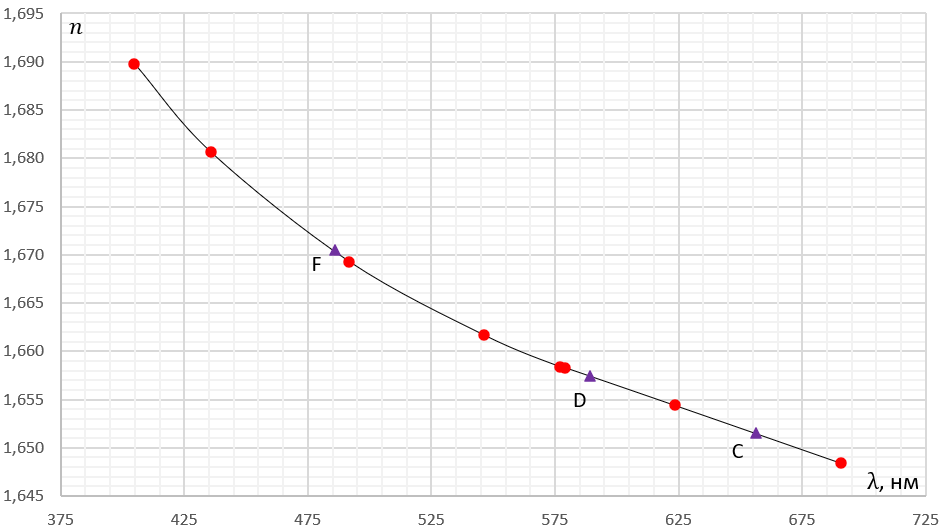
\includegraphics[width = 0.7\textwidth]{image/graph1.png}
        \caption{Дисперсионная кривая. Треугольниками обозначены точки F, D, C, соответствующие длинам волн $486,1$, $589,3$, $656,3$ нм соответственно}
    \end{figure}
    
\noindent По графику определим значения $n_D$ (жёлтый дублет натрия), $n_F$ (голубая линия водорода) и $n_C$ (красная линия водорода)

\begin{table}[!ht]
    \centering
    \begin{tabular}{|c|c|c|}
    \hline
    $n_D$  & $n_F$  & $n_C$  \\ \hline
    $1,4704 \pm 0,0001$ & $1,4724 \pm 0,0001$ & $1,4687 \pm 0,0001$ \\ \hline
    \end{tabular}
    \end{table}

\noindent Рассчитаем среднюю дисперсию оптического стекла $$D = n_F - n_C = 0,0037 \pm 0,0002$$ и коэффициент дисперсии $$\nu = \frac{n_D - 1}{n_F - n_C} = 125 \pm 5.$$ По наклону прямой $|\frac{dn}{d\lambda}| = 2,4 \cdot 10^3$ см$^{-1}$ рассчитаем максимальную разрешающую способность призмы $$R = b\frac{dn}{d\lambda} \approx (1,776 \pm 0,002)\cdot 10^4.$$

\noindent Для оценки разрешающей способности призмы воспользуемся табл. 3 и сопроводительным рисунком (рис. 3).

\begin{table}[!ht]
    \centering
    \caption{Измерение угловой ширины жёлтых линий дублета}
    \begin{tabular}{|c|c|c|c|}
    \hline
    $x_0$     & $x_1$    & $x_2$    & $x_3$    \\ \hline
    $7' 14''$ & $6'40''$ & $5'53''$ & $5'23''$ \\ \hline
    \end{tabular}
    \end{table}

\begin{figure}[ht!]
    \centering
    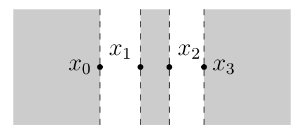
\includegraphics[width = 0.3\textwidth]{image/pic2.png}
    \caption{Измерение угловой ширины жёлтых линий дублета}
\end{figure}

\noindent Рассчитаем экспериментальную величину $R$ по измерениям жёлтого дублета $$R > \frac{d\lambda}{\lambda} \approx 275.$$

\noindent Рассчитаем угловую дисперсию $$\frac{d\phi}{d\lambda} = 0,0126 \pm 0,0006 \;\text{нм}^{-1}$$ и сравним её с дисперсией решётки в первом порядке, имеющей 100 штр/мм: $$D = 5,73 \cdot 10^5 \;\text{нм}^{-1}.$$

\section{Вывод}

В ходе работы исследовали дисперсию света ртутной лампы на стеклянной призме. По измеренным данным определили показатели преломления для длин волн жёлтого дублета натрия, голубой и красной линий водорода. По графику, изображенному на рис. 2, можно определить марку стекла (по наклону). Полученное значение соответствует марке стекла ТФ3. Также с помощью графика была получена максимальная разрешающая способность призмы. Далее была исследована экспериментальная величина $R$ по измерениям жёлтого дублета. После чего была рассчитана угловая дисперсия, которую сравнили с дисперсией решётки в первом порядке.

\section{Приложение: графики}

\begin{figure}[ht!]
    \centering
    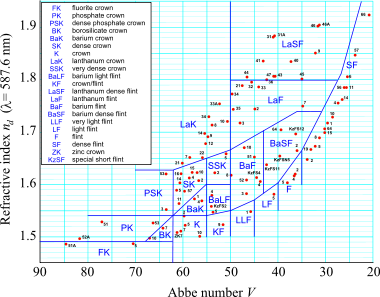
\includegraphics[width = 0.7\textwidth]{image/pic3.png}
    \caption{Диаграмма Аббе}
\end{figure}

\end{document}
